\documentclass{report}
\usepackage{graphicx} % Required for inserting images
\usepackage[italian]{babel}
\usepackage{tikz}
\usepackage{hyperref}
\usepackage{amsmath}
\usepackage{xcolor}
\usepackage{float}

\definecolor{darkgreen}{rgb}{0.0, 0.5, 0.0}


\title{Tastiera, Schermi, Palmo touchless}
\date{Parte X}

\begin{document}

\maketitle

\tableofcontents
\newpage

\chapter{Biometria della digitazione
della tastiera e schermi}

\section{\textit{Keystroke dynamics}}

I sistemi di identificazione basati sulla dinamica della battitura della tastiera 
(\textit{Keystroke dynamics}) si basano sull'assunzione che \textbf{persone 
diverse battano la tastiera in modi diversi}.

L'analisi della digitazione e della firma online sono simili:
\begin{itemize}
    \item tratti biometrici \textbf{comportamentali}
    \item \textbf{variabili} nel tempo e in base alle condizioni dell'individuo
    \item considerati \textbf{poco invasivi}
    \item acquisibili con sensori \textbf{economici}
    \item tecniche di matching simili, richiedono \textbf{allineamenti temporali} 
\end{itemize}

\subsubsection{Autenticazione a due fattori}
La possibilità di estrarre il template direttamente intanto 
che viene digitato la password di fatto rende possibile 
una istantanea identificazione a due fattori.

\subsection{Estrazione delle feature}
\subsubsection{Feature locali}
Le feature locali che si possono estrarre sono tipicamente
le seguenti:
\begin{itemize}
    \item tempo di \textbf{latenza} fra due pressioni
    \item tempo di \textbf{battitura} del tasto (quanto rimane premuto)
\end{itemize}

\noindent Altre feature meno interessanti, ma che possono essere usate
a corredo delle precedenti, sono:
\begin{itemize}
    \item velocità di battitura
    \item frequenza degli errori
    \item uso di \textit{shift} o \textit{caps lock}
\end{itemize}

\begin{figure}[ht]
    \centering
    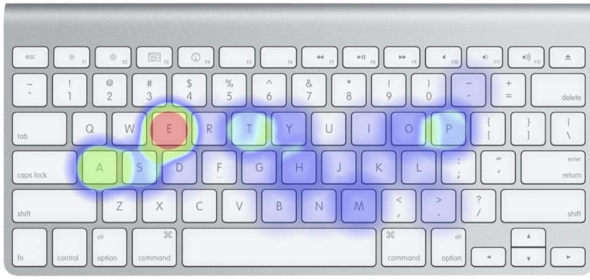
\includegraphics[width=0.8\linewidth]{images/tastiera-locali.png}
\end{figure}

\subsubsection{Feature globali}
Esistono anche delle feature globali, ovvero che si possono estrarre
solo quando la sessione di battitura è finita.


\noindent Si tratta delle \textbf{associazioni di tasti} (ad esempio,
quante viene usata la coppia ALT + TAB, o il tempo medio che intercorre
tra la loro battitura).


\section{Swapping su schermo}
Allo stesso modo, persone diverse hanno movimenti delle dita 
sullo schermo diversi.

\begin{figure}[H]
    \centering
    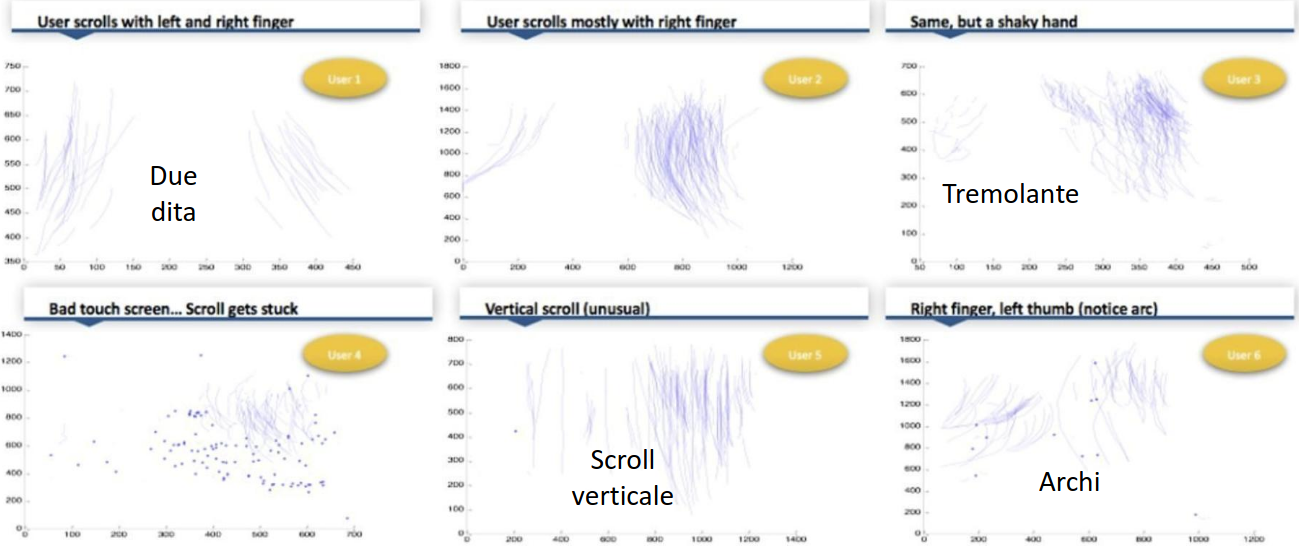
\includegraphics[width=1\linewidth]{images/schermo.png}
\end{figure}

\section{Comportamento dell'utente sul terminale}
In aggiunta, esistono dei metodi che vanno ad identificare
le persone in base al comportamento in:
\begin{itemize}
    \item ambiente software 
    \item rispetto al sistema operativo
\end{itemize}


\noindent Ad esempio, si può analizzare come viene usata la tastiera o il mouse,
come si passa da un'applicazione ad un'altra, come si accede ai menu, \dots

$\rightarrow$ con il solo comportamento \textbf{non è sempre possibile, usando questi metodi,
verificare l'identità di una persona} (troppa poca informazione).

\noindent Tuttavia, è possibile ricavare informazioni utili (ad esempio,
se durante il lavoro il terminale è usato proprio da quella persona o da un'altra).


\section{Vantaggi e Svantaggi}
\begin{itemize}
    \item \textcolor{darkgreen}{\textbf{Vantaggi}}
    \begin{itemize}
        \item Per regolare l'accesso dei terminali non è necessario un sensore, ma basta la tastiera del terminale; i sistemi sono quindi di tipo software
        \item Sono considerati non invasivi (anche se lo sono per la privacy)
        \item Possono essere impiegati anche senza la collaborazione dell'utente, o 
        addirittura senza che se ne accorga
    \end{itemize}
    \item \textcolor{red}{\textbf{Svantaggi}}
    \begin{itemize}
        \item \textbf{bassa} accuratezza
        \item queste informazioni possono essere usate per migliorare i tempi di \textbf{rottura delle password}
        \item \textbf{cambiando tastiera}, spesso i tempi cambiano, oppure solo impugnando qualcosa con l'altra mano
        \item \textbf{ferite o traumi} sulla mano possono influenzare la battitura
    \end{itemize}
\end{itemize}

\newpage
\section{Attacco su canale SSH}
È possibile perché esistono protocolli, come SSH, che trasmettono immediatamente 
un pacchetto ogni volta che viene premuto un tasto; in questo 
modo è possibile intercettare la password e i tempi di latenza.

\noindent I tempi di latenza non bastano per estrarre immediatamente
la password, ma permettono ai motori di generazione delle password
di ridurre i tempi di calcolo.

\subsection{Contromisure}
L'idea è di offuscare i dati che passano attraverso il canale SSH:
\begin{itemize}
    \item \textbf{Randomizzazione temporale:} viene introdotto un ritardo casuale per l'invio dei pacchetti 
    \item \textbf{Iniezioni di pacchetti \textit{dummy}}: pacchetti vuoti o non necessari, per alterare il ritmo di trasmissione 
    \item \textbf{Aggregazione di pacchetti:} si aggregano più pacchetti in un solo, per eliminare la correlazione diretta tra 
    i tempi di battitura e i tempi di invio
\end{itemize}

\chapter{Impronta}

\section{Biometria \textit{less-constrained} e \textit{unconstrained}}

\begin{itemize}
    \item \textit{Less-constrained}
    \begin{itemize}
        \item senza contatto
        \item elevata distanza
        \item condizioni di luce naturale
        \item in movimento
        \item \dots
    \end{itemize}
    $\rightarrow$ serve un minimo di cooperazione

    \item \textit{Unconstrained}
    \begin{itemize}
        \item soggetti non cooperativi
        \item scenari non controllati
    \end{itemize}
\end{itemize}

\newpage
\section{Vantaggi e Svantaggi}

\begin{itemize}
    \item \textcolor{darkgreen}{\textbf{Vantaggi}}
    \begin{itemize}
        \item less-constrained
        \item assenza di distorsioni della pelle nelle immagini delle dita 
        \item più resistente a sporco e polvere 
        \item maggiore accettazione da parte degli utenti
    \end{itemize}
    \item \textcolor{red}{\textbf{Svantaggi}}
    \begin{itemize}
        \item parzialmente compatibile con i sistemi AFIS
        \item sfondi complessi da gestire 
        \item sensibile ad illuminazione e posizione (vicino/lontano)
        \item i modelli 2D possono presentare distorsioni di tipo prospettico
        \item tempo di calcolo più lunghi
    \end{itemize}
\end{itemize}

\begin{figure}[ht]
    \centering
    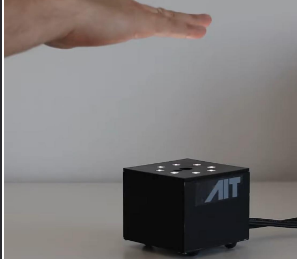
\includegraphics[width=0.6\linewidth]{images/finger.png}
\end{figure}

\chapter{Palmo}


\begin{figure}[ht]
    \centering
    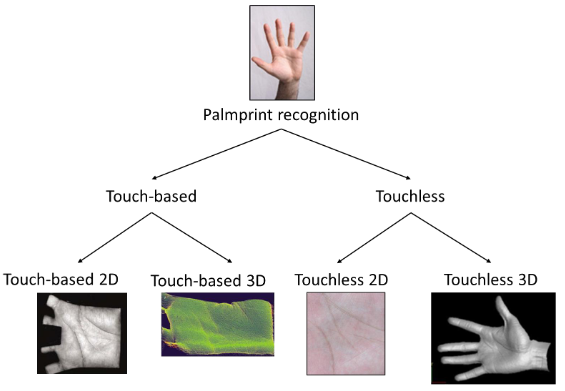
\includegraphics[width=1\linewidth]{images/palmo.png}
\end{figure}

\noindent L'area di lavoro tipicamente va dal polso 
alla base/punta delle dita.

\newpage
\section{Feature e matching}

Tra le feature estratte troviamo:
\begin{itemize}
    \item Point based
    \begin{itemize}
        \item delta points 
        \item se visibili, feature ereditate dalle impronte digitali 
    \end{itemize}
    \item Ridge based
    \begin{itemize}
        \item ridge principali 
    \end{itemize}
    \item Subspace-based (globali)
    \begin{itemize}
        \item basate su PCA 
    \end{itemize}
    \item Statistical 
    \item Coding-based
\end{itemize}

\noindent I moduli di matching sono ad-hoc in base al modulo di estrazione 
delle feature utilizzato, da una semplice metrica euclidea, fino a funzioni
complesse e \textit{deep}.

\begin{figure}[ht]
    \centering
    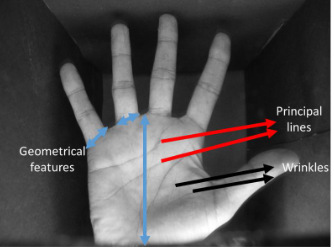
\includegraphics[width=0.8\linewidth]{images/palm-feature.png}
\end{figure}

\newpage
\section{2D palmprint touch}
\begin{itemize}
    \item approccio simile alle impronte 
    \item spesso gli scanner sono multifunzionali e possono acquisire anche impronte a contatto 
    \item si lasciano le tracce delle impronte sullo scanner
\end{itemize}

\begin{figure}[ht]
    \centering
    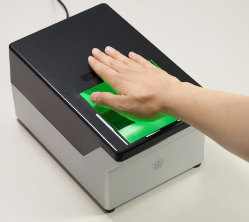
\includegraphics[width=0.5\linewidth]{images/2d-palm-touch.png}
\end{figure}

\section{2D palmprint touchless}

\begin{itemize}
    \item tendono ad avere minore o uguale accuratezza rispetto ai sistemi a contatto 
    \item i template estratti non sono comptabili con le tecnologie a contatto 
    \item maggiore usabilità 
    \item \textbf{non lascia traccia di impronte}
    \item tecnologie IR per vene e 
\end{itemize}

\subsubsection{\textcolor{darkgreen}{Vantaggi}}

\begin{itemize}
    \item less-constrained
    \item risoluzioni basse 
    \item maggiore accettabilità da parte dell'utente
    \item nessuna traccia sul dispositivo 
    \item robusto a dispersione e sporco 
    \item multibiometrico (combinazione con impronta, forma dita, forma mano, \dots)
\end{itemize}

\subsubsection{\textcolor{red}{Svantaggi}}

\begin{itemize}
    \item funzionalità ad alta precisione non sempre utilizzabili (minuzie II livello)
    \item basso contrasto e sfondi complessi; può diventare un problema in ambiente non controllato
    \item sensibile all'illuminazione 
    \item sensibile alla posizione, rischia di rendere l'immagine non a fuoco 
\end{itemize}

\begin{figure}[ht]
    \centering
    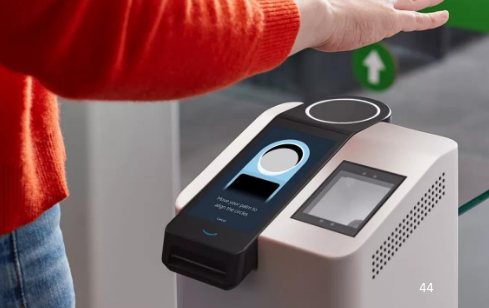
\includegraphics[width=0.7\linewidth]{images/palm-touchless-2d.png}
\end{figure}


\section{2D touchless vein palmprint (IR)} 

Categoria particolare dove non si guardano le classiche feature di livello
1 e 2 della epidermide, ma la distribuzione delle vene visibili in infrarosso.

\begin{figure}[ht]
    \centering
    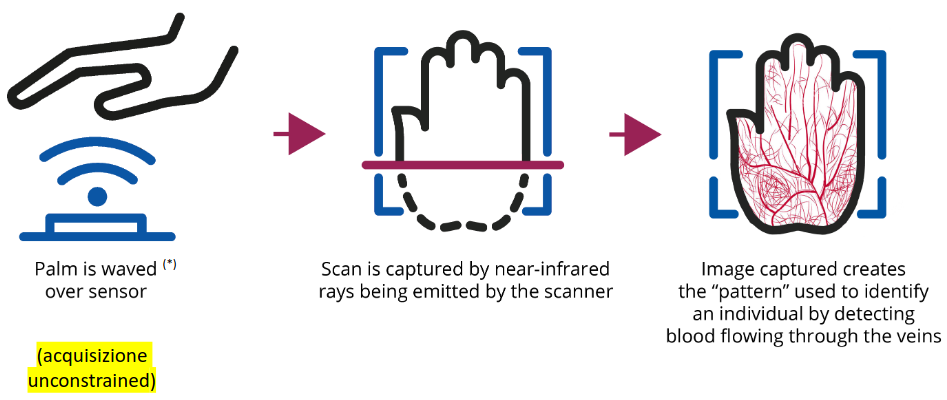
\includegraphics[width=1\linewidth]{images/vein.png}
\end{figure}

\newpage
\section{Acquisizione del palmo 3D}

\begin{itemize}
    \item \textcolor{darkgreen}{\textbf{Vantaggi}}
    \begin{itemize}
        \item robusto per illuminazione, occlusioni, rumore 
        \item resistente ad attacchi di spoofing
        \item invariante a posizione e distanza
        \item può utilizzare anche informazioni 2D
    \end{itemize}
    \item \textcolor{red}{\textbf{Svantaggi}}
    \begin{itemize}
        \item dispositivo complesso 
        \item può essere costoso
    \end{itemize}
\end{itemize}

\begin{figure}[ht]
    \centering
    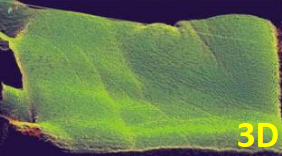
\includegraphics[width=0.8\linewidth]{images/3d-palm.png}
\end{figure}

\subsection{Sensori}

\noindent I sensori utilizzano:
\begin{itemize}
    \item \textbf{touch-based}
    \begin{itemize}
        \item luce strutturata
    \end{itemize}
    \item \textbf{touchless}
    \begin{itemize}
        \item laser
        \item multi-view
        
        $\rightarrow$  Per ottenere i dati 3D si può usare sia una telecamera che fa più acquisizioni nel tempo, 
        sia 2 telecamere che fanno una acquisizione mulipla
    \end{itemize}
\end{itemize}














\end{document}